\documentclass[10pt]{report}
\usepackage[utf8]{inputenc}
\usepackage[italian]{babel}
\usepackage{multicol}
\usepackage[bookmarks]{hyperref}
\usepackage[a4paper, total={18cm, 25cm}]{geometry}
\usepackage{graphicx}
\usepackage{xcolor}
\usepackage{textcomp}
\graphicspath{ {./img/} }
\usepackage{listings}
\usepackage{makecell}
\lstdefinestyle{customasm}{
  belowcaptionskip=1\baselineskip,
  frame=line,
  xleftmargin=\parindent,
  language=[x86masm]Assembler,
  basicstyle=\ttfamily,
  commentstyle=\itshape\color{purple!40!black},
}
\lstset{escapechar=@,style=customasm}
\lstnewenvironment{C}
  {\lstset{language=C++,frame=none}}
  {}
\begin{document}
\title{Machine Learning}
\author{Federico Matteoni}
\date{A.A. 2021/22}
\renewcommand*\contentsname{Index}

\maketitle
\begin{multicols}{2}
\tableofcontents
\end{multicols}
\pagebreak
\section{Introduction}
What is ML? Area of research combining aims of creating computers that could learn and powerful and adaptive statistical tools with rigorous foundation in computational science. Luxury or necessity? Growing availability and need for analysis of empirical data and difficult to provide intelligence and adaptivity by programming it. Change of paradigm.\\
Examples: spam classification, written text recognition\ldots No or poor prior knowledge and rules for solving the problem, but easier to have a source of training experience.\\
ML is considered the latest general-purpose technology, capable of drastically affect pre-existing economic and social structures. And already has. The ultimate aim is to bring benefits to the people by solving big and small problems, accelerating human progress and empowering humans to add intelligence in any other science field.
\paragraph{Machine Learning} We restrict to the computational framework: principles, methods and algorithms for learning and prediction, from experience. Building a model to be used for predictions. Common framework: infer a model or a \textbf{function} from a set of examples which allows the generalization (accurate response to new data).\\
When can we use ML? Be aware of the opportunity and awareness. ML is useful when there's no or poor theory surrounding the phenomenon, or uncertain, noisy or incomplete data which hinders formalization of solutions. The requests are: source of training experience (representative data) and a tolerance on the precision of results. The best examples are models to solve real-world problems that are difficult to be treated with traditional techniques: face and voice recognition (knowledge too difficult to formalize in an algorithm), predicting biding strength of molecules to proteins (not enough human knowledge) and personalized behavior, such as recommendation systems, scoring messages according to user preferences\ldots
\paragraph{Definition} The ML studies and proposes methods to build functions/hypothesis from examples of observed data that fits the known examples and able to generalize, with reasonable accuracy, for new data (according to verifiable results and under statistical and computational conditions and criteria.
\paragraph{Data} Data \textbf{represents the available experience}. Representation problem: capturing the structure of the analyzed objects. Flat (attribute-value), structured\ldots, categorical or continuous, missing data\ldots \textbf{preprocessing}: variable scaling, encoding, selection\ldots
\paragraph{Task} The task defines the purpose of the application: knowledge that we want to achieve? which is the helpful nature of the result? what information are available?\\
\textbf{Predictive} task, classification and regression: function approximation\\
\textbf{Descriptive} task, cluster analysis and association rules: find subsets or groups of unclassified data.
\begin{center}
	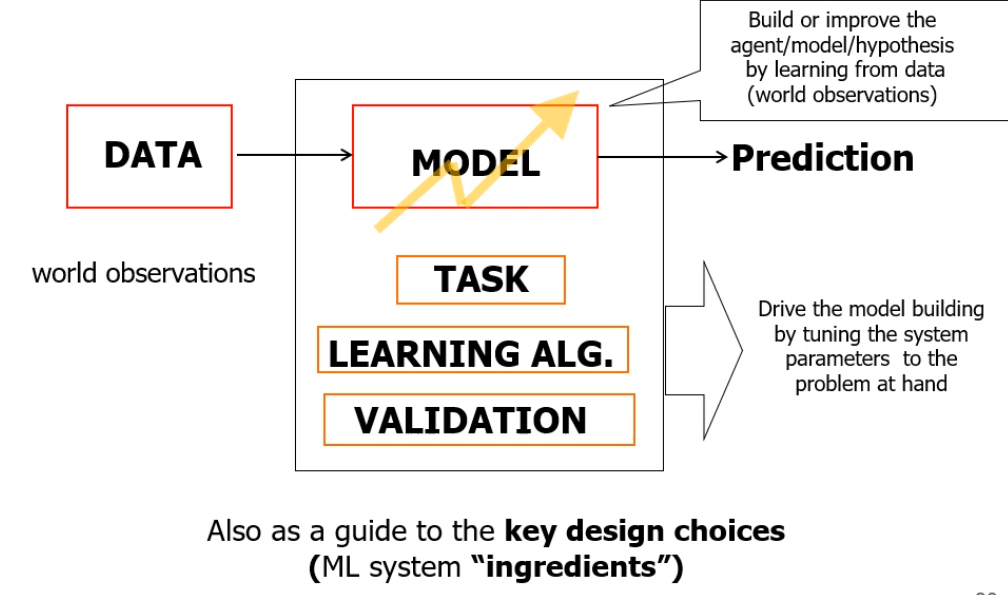
\includegraphics[scale=0.5]{1.png}
\end{center}
\pagebreak
\paragraph{Supervised learning} Given a set of training examples as $\langle$input, output$\rangle$ = $\langle x,d\rangle$ (\textbf{labeled examples}) for an unknown function $f$, find a \textit{good approximation} of $f$, an hypothesis $h$ that can be used for making predictions on unseen data $x'$.\\
The target $d$ can be:
\begin{list}{}{}
	\item Discrete value, for \textbf{classification tasks}.\\
	$f(x) \in \{1,2,\ldots,k\}$\\
	Patterns, feature vectors, are seen as members of a class and the goal is to assign the new patterns observed to the correct class (or label)\\
	If the number of possible classes is two, then $f$ is a \textit{boolean function} and the task is called \textbf{binary classification} or \textbf{concept learning}: true or false, positive or negative, 0 or 1\ldots\\
	If the number of classes is greater that two then is a \textbf{multi-class classification task}.
	\item Real continuous value, for \textbf{regression tasks}.\\
	The patterns are seen as sets of variables (real values), and the task is a curve fitting task. The process aims to estimate a real-value function based of a finite set of noisy samples $\langle x, f(x) +$ random noise$\rangle$
\end{list}
\paragraph{Unsupervised learning} No teacher. The training set is a set of unlabeled data $\langle x\rangle$. Examples: clustering, finding natural groupings in a set of data.
\paragraph{Learning algorithm} Basing on data, task and model: heuristic search through the hypothesis space $H$ of the \textbf{best hypothesis}. I. e. the best approximation of the unknown target function, typically searching for the $h$ with the minimum \textit{error}. $H$ may not coincide with the set of all possible function and the search cannot be exhaustive, we need to make \textbf{assumpitons} (\textbf{inductive bias}).
\paragraph{Learning} Also called:
\begin{list}{}{}
	\item Inference, in statistics
	\item Adapting, in biology and systems
	\item Optimizing, in mathematics
	\item Training, in neural networks
	\item Function approximations, in mathematics
	\item \ldots
\end{list}
After introducing data, task, model and learning algorithm we will focus on: inductive bias, loss and concepts of generalization and validation.
\paragraph{Inductive bias} To set up a model we can make assumptions about the nature of the target function, concerning either:
\begin{list}{}{}
	\item constraints in the model, \textbf{language bias} (in the hypothesis space $H$, due to the set of hypothesis that we can express or consider
	\item constraints or preferences in learning algorithm/search strategy, \textbf{search bias} which is preferred
	\item or both
\end{list}
Such assumptions are needed to obtain an useful model for the ML aims, i.e. a model with generalization capabilities.\\
We can imagine learning a discrete function with discrete inputs assuming \textbf{conjunctive rules}, so using a \textbf{language bias} to work with a restricted hypothesis space.
\paragraph{Version Space} An hypothesis $h$ is consistent with the TR if $h(x) = d(x)$ for each training example $\langle x, d(x)\rangle$.\\
The \textbf{version space} $VS_{H, TR}$ is the subset of $H$ of the hypothesis consistent with all the training examples $\langle x, d(x)\rangle$ in the TR.\\
It's possible to do an exhaustive search in an efficient way, using clever algorithms. This means finding the set of all the hypothesis $h$ consistent with the TR set. 
\paragraph{Unbiased Learner} The language bias (ex: using only conjunctive rules, may be too restrictive: if the target concept is not in $H$ it cannot be represented in $H$. We can use an $H$ that expresses every teachable concept (among propositions), that means that $H$ is the set of all possible subsets of $X$: the power set $P(X)$. If $n = 10$ binary inputs, then $|X| = 2^{10} = 1024$ and $|P(X)| = 2^{1024} = 10^{308}$ possible concepts, which is much more than the number of the atoms in the universe.\\
An unbiased learner is unable to generalize: the only examples that are unambiguously classified by an unbiased learner represented with the VS are the training examples themselves. Each unobserved instance will be classified positively by exactly half of the hypothesis in the VS and negative by the other half. Indeed: $\forall\: h$ consistent with $x_i$, $\exists\:h'$ identical to $h$ except $h'(x_i) \neq h(x_i)$, $h\in$ VS $\Rightarrow h'\in$ VS (because they are identical on the TR)\\\\
Why prefer the search bias? In ML we use flexible approaches (expressive hypothesis spaces with universal capability of the models, for example neural networks or decision trees. We avoid the language bias, so we do not exclude a priori the unknown target function, but we focus on the search bias (ruled by the learning algorithm).
\paragraph{Loss} How to measure the quality of an approximation? We want to measure the distance between $h(x)$ and $d$, using a loss function/measure $L(h(x), d)$ for a pattern $x$ which has high value in cases of bad approximation. The error (or risk or loss) is an expected value of this $L$, for example $E(w) = \frac{1}{l}\sum_{p=1}^l L(h(x_p), d_p)$. Different $L$ for different tasks. Examples of loss functions:
\begin{list}{}{}
	\item Regression: $L(h(x_p), d_p) = (d_p - h(x_p))^2$, the squared error. MSE (mean squared error) over the data set
	\item Classification: $L(h(x_p), d_p) = \left\{\begin{array}{l l}
		0 & h(x_p) = d_p\\
		1 & else
	\end{array}\right.$
\end{list}
\paragraph{Learning and generalization} Learning: search for a \textbf{good function} in a function space from known data (typically minimizing an error/loss). \textbf{Good} with respect to generalization error: it measures how accurately the model predicts over novel samples of data (\textbf{measured over \underline{new} data}).\\
Generalization is the crucial point of ML. Performance in ML is the generalization accuracy or \textit{predictive accuracy} estimated by the error on the test set.
\paragraph{ML issues} Inferring general functions from known data is an ill posed problem, which means that in general the solution is not unique because we can't expect the exact solution with finite data. What can we represent? And so, what can we learn?\\
Learning phase: building the model including training. The prediction phase is evaluating the learned function over new never-seen-before samples (generalization capability). Inductive learning hypothesis: any $h$ that approximates $f$ well on training examples will also approximate $f$ well on new unseen instances $x$.\\
\textbf{Overfitting}: a learner overfits data if it outputs an hypothesis $h\in H$ having true/generalization error (risk) $R$ and empirical (training) error $E$, but there's another $h'\in H$ with $E' > E$ and $R' < R$, which means that $h'$ is the better one despite having a worse fitting.
\paragraph{Statistical Learning Theory} Under what mathematical conditions is a model able to generalize? We want to investigate the generalization capability of a model, measured as a risk or test error, the role of the model complexity and the role of the number of data.\\
\textbf{Formal Setting}: approximate a function $f(x)$, with $d$ target ($d = f(x) +$ noise), minimizing the \textbf{risk function} $$R = \int L(d, h(x))\:dP(x,d)$$ which is the \textbf{true error over all the data}, given:
\begin{list}{}{}
	\item a value $d$ from the teacher and the probability distribution $P(x,d)$
	\item a loss function $L(h(x),d) = (d - h(x))^2$
\end{list}
We search for $h\in H\:|\: min\:R$, but we only have the finite data set $TR = (x_p, d_p)$ with $p = 1\ldots l$. Looking for $h$ means minimizing the empirical risk (the training error $E$), finding the best values for the model free parameters $$R_{emp} = \frac{1}{l}\sum_{p=1}^l (d_p - h(x_p))^2$$
The inductive principle is the \textbf{ERM}, Empirical Risk Minimization: can we use $R_{emp}$ to approximate $R$?
\paragraph{Vapnik-Chervoneniks dim and SLT} Given the VC dimension (simply VC), a measure of complexity of $H$ and by that we mean its flexibility to fit data.\\
The VC-bound states that it holds with probability $\frac{1}{\delta}$ that $$R \leq R_{emp} + \epsilon\left(\frac{1}{l}, \textsl{VC},\frac{1}{\delta}\right)$$
\begin{list}{}{}
	\item $\epsilon$ is a function called VC-confidence, that grows with VC and decreases with higher $l$ and $\delta$
	\item $R_{emp}$ decreases using complex models (with high VC)
	\item $\delta$ is the confidence, and it rules the probability that the bound holds.\\
	$\delta = 0.01 \Rightarrow$ the bound holds with probability $0.99$
\end{list}
Intuitively:
\begin{list}{}{}
	\item Higher $l$ (data) $\Rightarrow$ lower VC confidence and bound closer to $R$
	\item A too simple model, meaning with low VC, can be not sufficient due to high $R_{emp}$ (\textbf{underfitting})
	\item An higher VC with fix $l \Rightarrow$ lower $R_{emp}$ but VC and hence $R$ may increase (\textbf{overfitting})
\end{list}
\paragraph{Structural risk minimization} Minimize the bound! There are different bounds formulations according to different classes of $f$, of tasks\ldots\\
In other words, we can make a good approximation of $f$ from examples, provided that we have a good number of data and the complexity of the model is suitable for the task.
\paragraph{Complexity control} The Statistical Learning Theory allows for a formal framing of the problem of generalization and overfitting, providing an analytic upper bound to the risk $R$ for the prediction over all the data, regardless of the type of learning algorithm or the details of the model. So \textbf{the machine learning is well founded}, the learning risk can be analytically limited and only a few concepts are fundamental. This leads to new models (such as the Support Vector Machine) and other methods that directly consider the control of the complexity in the construction of the model.
\paragraph{Validation} Central role for the applications and the project. Two aims:
\begin{list}{}{}
	\item \textbf{Model Selection}: estimating the performance (\textbf{generalization error}) of different models in order to choose the best one. This includes searching for the best hyperparameters of the model.\\
	It returns a model.
	\item \textbf{Model Assessment}: with the final model, estimating/evaluating its prediction error/risk (\textbf{generalization error}) over new test data.\\
	It returns an estimation.
\end{list}
\textbf{Golden rule}: keep the two goals separated and use different datasets for each one.\\\\
In an ideal world, we'd have a large training set, a large validation set for model selection and a very large external unseen data test set. With finite and often small data sets we have just an estimation of the generalization performance. We have to use some techniques: hold-out and k-fold cross validation, for example.
\begin{list}{}{}
	\item \textbf{Hold-Out}: we partition the dataset $D$ into \textbf{training set} TR, \textbf{validation/selection set} VL and \textbf{test set} TS.\\
	All three are disjoint: TR is used to run the training algorithm, VL can be used to select the best model (hyperparameters tuning) and the \textbf{TS is only used for model assessment}.
	\begin{center}
		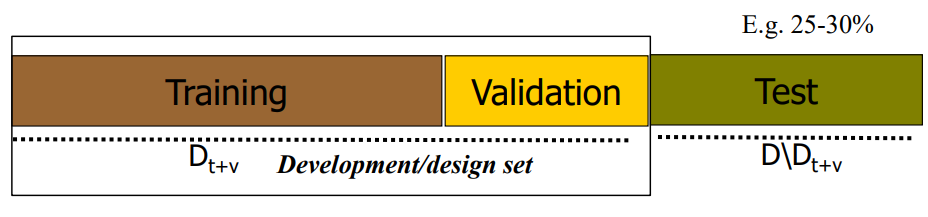
\includegraphics[scale=0.5]{2.png}
	\end{center}
	\item \begin{multicols}{2}
	\textbf{K-Fold}: this technique can make use of insufficient data. We split the dataset $D$ into $k$ mutually esclusive subsets $D_1,\ldots, D_k$, we train on $D - D_i$ and test it on $D_i$.\\
	This can be applied to both VL and TS splitting. Can be computationally very expensive and there's the issue of choosing the number of folds $k$.
	\begin{center}
		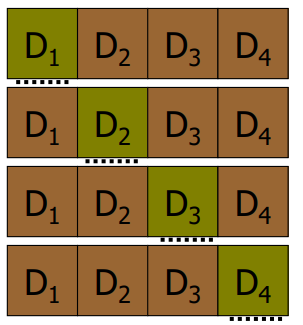
\includegraphics[scale=0.5]{3.png}
	\end{center}
	\end{multicols}
\end{list}
\paragraph{Confusion Matrix} \begin{center}
	\begin{tabular}{|c|c|c|}
		\hline
		Actual/Predicted & \textbf{Positive} & \textbf{Negative}\\
		\hline
		\textbf{Positive} & TP & FN\\
		\hline
		\textbf{Negative} & FP & TN\\
		\hline
	\end{tabular}
\end{center}
\textbf{Specificity} = $\frac{\textsl{TN}}{\textsl{FP} + \textsl{TN}}$, and \textbf{true negative rate} $= 1 - \textsl{FPR}$\\
\textbf{Sensitivity} = $\frac{\textsl{TP}}{\textsl{TP} + \textsl{FN}}$, also known as \textbf{true positive rate} or \textbf{recall}\\
\textbf{Precision} = $\frac{\textsl{TP}}{\textsl{TP} + \textsl{FP}}$\\
\textbf{Accuracy}: \% of correctly classified patterns = $\frac{\textsl{TP + TN}}{\textsl{total}}$. Note that, for example, a 50\% accuracy on a binary classifier is equivalent to a random predictor.
\paragraph{ROC Curve} We plot \textbf{specificity} on \textbf{x-axis} and \textbf{sensitivity} on the \textbf{y-axis}. The diagonal corresponds to the worst classifier, the random guesser. Better curves have greater Area Under the Curve (AUC)
\paragraph{Linear Models} Mainstay of statistics.
\subparagraph{Univariate Linear Regression} Simple linear regression: we start with 1 input variable $x$ and 1 output variable $y$. We assume a model $h_w(x)$ expressed as $out = w_1x + w_0$ where $w$ are real-valued coefficients or \textbf{free parameters}, also called \textbf{weights}.\\
Given that the $w$s are continuous valued, we have an infinite hypothesis space but a nice solution from classical math. We can learn with this basic tool and, although simple, it includes many relevant concepts of modern ML and many methods in the field are based on this.\\
\textbf{Least Mean Square}: learning means finding $w$ such that it minimizes the error/empirical loss, with best data fitting on the training set with $l$ examples.\\
So given a set of $l$ training examples $(x_p, y_p)$ with $p = 1,\ldots,l$, we have to find $h_w(x)$ in the form $w_1x + w_0$ that minimizes the expected loss on the training data. For the loss, we use the square of errors: \textbf{least mean square}, find $w$ to \textbf{minimize} the residual sum of squares.
$$Loss(h_w) = E(w) = \sum_{p=1}^l (y_p - h_w(x_p))^2 = \sum_{p=1}^l (y_p - (w_1x_p + w_0))^2$$
To have the mean, divide by $l$. How to solve? Local minimum as stationary point, so the gradient $\frac{\partial E(w)}{\partial w_i} = 0$ with $i = 1,\ldots,$ dim\_input $+1 = 1,\ldots, n+1$. For the simple linear regression (2 free parameters):
$$\frac{\partial E(w)}{\partial w_0} = 0\:\:\:\:\frac{\partial E(w)}{\partial w_1} = 0$$
$$\frac{\partial E(w)}{\partial w_0} = -2(y - h_w(x))\:\:\:\:\frac{\partial E(w)}{\partial w_1} = -2(y - h_w(x))\cdot x$$
\subparagraph{Classification} The same models used for regression can be used for classification: \textbf{categorical targets} $y$ or $d$, for example 0/1, -1/+1\ldots\\
We use an hyperplane ($wx$) assuming negative or positive values. We exploit such models to decide if a point $x$ belongs to the positive or the negative zone of the hyperplane to classify it. So we want to learn $w$ such that we get a good classification accuracy. The decision boundary is $x^Tw = w^Tx = w_0 + w_1x_1 + w_2x_2 = 0$ and we can introduce a threshold function which can be written in many ways: \begin{list}{}{}
	\item $h(x) = \left\{\begin{array}{c l}
	1 & \textsl{if }wx + w_0 \geq 0\\
	0 & \textsl{else}
\end{array}	 \right.$
	\item $h(x) = \textsl{sign}(wx + w_0)$
	\item \ldots
\end{list}
$w_0$ is called \textbf{threshold} or \textbf{bias}. $h(x) = w^Tx + w_0 \geq 0 \Leftrightarrow w^Tx \geq -w_0$
\paragraph{Learning Algorithms} Introducing 2 learning algorithms, both based on LSM and used for the linear model on regression and classification tasks. We start redefining the learning problem and the loss for them (in the case of $l$ data and multidimensional inputs).\\\\
\textbf{Learning problem for classification tasks}: given a set of $l$ training examples $(x_p, y_p)$ and a loss function $L$, with $y_p \in \{0,1\}$ or $y_p \in \{-1, +1\}$, find the weight vector $w$ that minimizes expected loss on the training data $$R_{emp} = \frac{1}{l}\sum_{p=1}^l L(h(x_p), y_p)$$
The expected loss can be approximated by a smooth function. We can make the optimization problem easier by replacing the original objective function $L$ (0/1 loss) with a smooth, differentiable function: for example, the MSE loss (mean squared error).
\begin{center}
	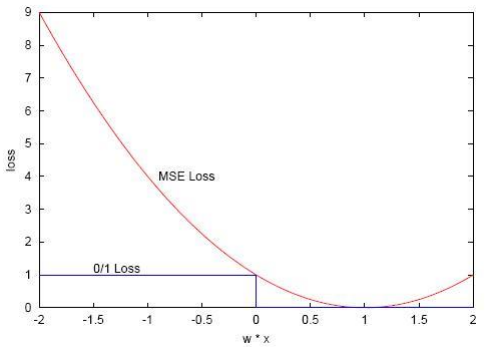
\includegraphics[scale=0.75]{4.png}
\end{center}
No classification error minimizing either 0/1 loss or MSE loss. Given $l$ training examples $(x_p, y_p)$, find $w$ that minimizes the residual sum of squares $$E(w)= \sum_{p=1}^l (y_p - x_p^T w)^2 = ||y - Xw||^2$$
We can't use $h(x)$ in $E(w)$, as for regression, because $h(x) = \textsl{sign}(w^T x)$ is non-differentiable. Also, this is a quadratic function so the minimum always exists (but may not be unique). $X$ is a $l\times n$ matrix with a row for each $x_p$.
\subparagraph{Direct Approach with a normal equation} Differentiating $E(w)$ with respect to $w$ to get the \textbf{normal equation} $$(X^T X)w = X^T y$$
In the derivation we also find that $$\frac{\partial E(w)}{\partial w_j} = -2 \sum_{p=1}^l (x_p)_j \cdot (y_p - x_p^T w)$$
If $X^T X$ is not singular, then the unique solution is given by $$w = (X^T X)^{-1}X^T y = X^+ y$$ with $X^+$ being the Moor-Penrose pseudoinverse. Else the solutions are infinite, so we can choose the \textbf{min norm}$(w)$ solution.\\
The \textbf{Singular Value Decomposition} can be used for computing the pseudoinverse of a matrix ($X^+$). With\\ $X = U\Sigma V^T \Rightarrow X^+ = V\Sigma^+ U^T$ replacing every non-zero entry by its reciprocal. We can apply SVD directly to compute $w = X^+ y$, obtaining the minimal norm (on $w$) solution of least squares problem.
$$\frac{\partial E(w)}{\partial w_j} = \frac{\partial \sum_{p=1}^l (y_p - x_p^T w)^2}{\partial w_j} = \ldots = -2 \sum_{p=1}^l (y_p - x_p^T w)(x_p)_j$$
\paragraph{Gradient Descent} The derivation suggests an approach based on an iterative algorithm based on\\$\frac{\partial E(w)}{\partial w_j} = -2 \sum_{p=1}^l (y_p - x_p^T w)(x_p)_j$. The \textbf{gradient} is the \textbf{ascent direction}. We can move toward the minimum with a gradient descent $\Delta w = -$ gradient of $E(w)$. \textbf{Local search}: we begin with a initial weight vector and modify it iteratively to minimize the error function. The gradient vector is
$$\Delta w = -\frac{\partial E(w)}{\partial w} = \left[\begin{array}{c}
-\frac{\partial E(w)}{\partial w_1}\\\vdots\\-\frac{\partial E(w)}{\partial w_n}
\end{array}\right] = \left[\begin{array}{c}
\Delta w_1\\\vdots\\\Delta w_n
\end{array} \right]$$
Allowing us to work in a multi dimensional space without the need to visualize it. Hence, the iterative approach will move using a learning rule based on a "delta" of $w$ proportional to the opposite of the local gradient. The movements will be made according to $$w_{new} = w + \eta\cdot\Delta w$$
The simple algorithm is as follows:
\begin{enumerate}
	\item Start with weight vector $w_{initial}$ and fix $0 < \eta < 1$
	\item Compute $\Delta w = -$ gradient of $E(w) = -\frac{\partial E(w)}{\partial w}$ (or for each $w_i$)
	\item Compute $w_{new} = w + \eta\cdot\Delta w$ (or for each $w_i$)\\
	$\eta$ is the step size or \textbf{learning rate}
	\item Repeat from $2$ until convergence or $E(w)$ sufficiently small
\end{enumerate}
\subparagraph{Batch version} The gradient is the sum over all the $l$ patterns. Provides a more precise evaluation of the gradient over $l$ data. We upgrade the weight after the sum
$$\frac{\partial E(w)}{\partial w_j} = -2 \sum_{p=1}^l (y_p - x_p^T w)(x_p)_j$$
\subparagraph{Online/Stochastic version} We upgrade the weights with the error that is computed for each pattern. Hence, the second pattern output is based on weights already updated from the first and so on. In makes progress with each example it sees. Can be faster, but needs smaller $\eta$
$$\frac{\partial E_p(w)}{\partial w_j} = -2(y_p - x_p^T w)(x_p)_j = -\Delta_p w_j$$
\subparagraph{Gradient Descent as error correction delta rule} The error correction rule, also called Widrow-Hoff or delta rule, changes $w_j$ proportionally to the error (target $y$ $-$ output)
$$\Delta w_j = 2 \sum_{p=1}^l (x_p)_j (y_p - x_p^T w)$$
$$w_{new} = w + \eta\cdot\Delta w$$
We improve by learning on previous errors.\\\\
Gradient descent is a simple and effective local search approach to a LMS solution. It allows to search through an infinite hypothesis space, can be easily applied for continuous $H$ and differentiable losses and isn't only for linear models (also neural networks and deep learning models).\\
Many possible improvements (Newton, quasi-Newton methods, conjugate gradients\ldots)
\paragraph{Linear models}\begin{list}{}{}
	\item \textbf{Language bias}: $H$ is a set of linear functions.
	\item \textbf{Search Bias}: ordered search guided by the least squares minimization goal. For instance, we could prefer a different method to obtain a restriction on the values of parameters, achieving a different solution with other properties.
\end{list}
Shows that even for a simple model there are many possibilities. We still need a principled approach.
\subparagraph{Limitations} In geometry, two set of points are linearly separable in an $n$-dimensional space if they can be separated by a $(n-1)$-dimensional hyper-plane. In 2 dimensions, if they can be separated by a line, in 3 dimensions, by a plane\ldots\\
The linear decision boundary can provide exact solutions only for linearly separable sets of points.
\subparagraph{Extending the linear model} We can use transformed inputs, such as $x, x^2, x^3\ldots$ with a non-linear relationship between inputs and output, maintaining the learning machinery used so far. $$h_w(x) = w_0 + w_1 x + w_2 x^2 + \ldots + w_M x^M = \sum_{j=0}^M w_j x^j$$ \textbf{Linear basis expansion} (LBE) $$h_w(x) = \sum_{k=0}^K w_k\phi_k(x)$$ Augments the input vector with additional variables which are transformations of $x$ according to a function $\phi_k : R^n \rightarrow R$, so number of parameters $K > n$: linear in the parameters, so we can use the same learning algorithms as before.\\
Which $\phi$? Towards the dictionary approaches. Pro: can model more complicated relationships than linear, so it's more expressive. Cons: with large basis of functions, we easily risk overfitting, hence we require controlling the complexity (as in flexibility of the model to fit the data). How to do that? Many approaches:
\begin{list}{}{}
	\item \textbf{Ridge Regression} (or \textbf{Tikhonov Regularization}): smoothed model.\\
	Add constraints to the sum of value of $|w_j|$, penalizing models with high values of $|w|$ (so favoring sparse models, using less terms due to weights $w_j = 0$ or close)
	$$Loss(w) = \sum_{p=1}^l (y_p - x_p^T w)^2 + \lambda||w||^2$$ with $\lambda$ being the regularization hyper-parameter. It implements the control of the model complexity, leading to a model with less VC-dim with a trade-off controlled through a single parameter, $\lambda$.\\
	This uses $||\:||_2$
	\item Lasso uses $||\:||_1$
	\item Elastic nets uses both $||\:||_1$ and $||\:||_2$
\end{list}
\paragraph{Learning Timing} \begin{list}{}{}
	\item \textbf{Eager}: analyze data and construct an explicit hypothesis
	\item \textbf{Lazy}: store tr data and wait test data point, then construct an ad hoc hypothesis.
\end{list}
\paragraph{k-NN}
The algorithm is simple: store the training data and given and input $x$ find the $k$ nearest training examples $x_i$, then output the mean label.
\subparagraph{Voronoi Diagram} Each cell consists of point closer to $x$ than any other patterns. The segments are all points in plan equidistant to two patterns. It is implicitly used by K-NN.
\subparagraph{K-NN vs linear} Two extremes of the ML panorama:
\begin{center}
	\begin{tabular}{c c}
		Linear & K-NN\\
		Rigid (low variance) & flexible (high variance)\\
		Eager & Lazy\\
		Parametric & Instance-Based
	\end{tabular}
\end{center}
\subparagraph{Bayes Error Rate} If we know the density $P(x,y)$, we classify the most probable class, using the conditional distribution as: output the class $v\:|\:$ is $max\:P(v\:|\:x)$.\\
The error rate of this classifier (called the Bayes classifier) is called the Bayes error rate: the minimum achievable error rate given the distribution of the data. K-NN directly approximates this solution (majority vote in a nearest neighborhood) except that conditional probability is relaxed to conditional probability withing a neighbordhood and probabilities are estimated by training sample proportions
\subparagraph{Inductive bias of K-NN} The assumed distance tells us which are the most similar examples. The classification is assumed similar to the classification of the neighbors according to the assumed metric.
\subparagraph{Limitations} The computational cost is deferred to the prediction phase: makes the local approximation to the target function for each new example to be predicted.\\
Moreover, high retrieval cost: computationally intensive, in time, for each new input because computes the distance from the test sample to all stored vectors, so high cost in space too (all training data).\\
It provides a good approximation if we can find a significant set of data close to any $x$. Can fail when we have a lot of input variables (high $n$, high dimensionality) due to the curse of dimensionality:
\begin{list}{}{}
	\item \textbf{Hard to find nearby points} in high dimensions\\
	K-NN can fail in high dimensions because it becomes difficult to gather $K$ observation close to a target point $x_q$: near neighborhoods tend to be spatially large and estimates are no longer local
	\begin{center}
		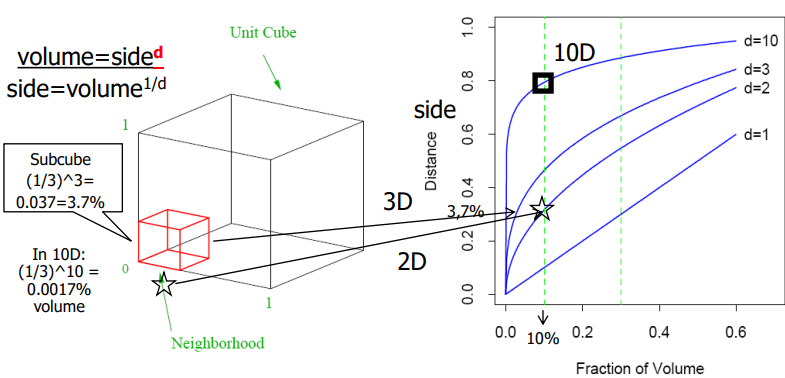
\includegraphics[scale=0.75]{5.png}
	\end{center}
	\item \textbf{Low sampling density} for high-dim data\\
	Sampling density is proportional to $l^{\frac{l}{d}}$ with $l$ data and $d$ data dim. If 100 points are needed to estimate a function in $R$ (1 dim), then $100^{10}$ are needed in $R^{10}$
	\item Irrelevant features: the \textbf{curse of noisy}\\
	If the target depends only on a few features in $x$, we could retrieve a similar pattern with the similarity dominated by the large number of irrelevant features.\\
	This grows with dimensionality.\\
	We may weight features according to the relevance, or adopt feature selection approaches (eliminating some variables)
\end{list}
% ML-21-NN-part1-v.0.1.pdf
\paragraph{Neural Networks} Models used to:
\begin{list}{}{}
	\item Study and model biological systems and learning processes (biological realism is essential)
	\item Introduce effective machine learning systems and algorithms (often losing a strict biological realism, but machine learning, computational and algorithmic properties are essential)
\end{list}
For us: \textbf{Artificial Neural Networks} (ANN): a flexible machine learning tool in the sens of approximating functions (builds a mathematical function $h(x)$ with special properties). A neural network:
\begin{list}{}{}
	\item Can learn from examples
	\item Are universal approximators (\textbf{Theorem of Cybenko}): flexible approaches for arbitrary functions (including non-linear)
	\item Can deal with noisy and incomplete data, with a graceful degradation of performance
	\item Can handle continuous real and discrete data for both regression and classification tasks
	\item It's a \textbf{paradigm}: it encompasses a wide set of models.
\end{list}
\paragraph{Artificial Neuron} Input from external source or other units, with weights $w$ as free parameters: can be modified by the learning process. The unit $i$ computes $f(\sum_j w_{ij}x_j)$ with $w_{ij}$ the weight from input $j$ to unit $i$. $f$ is called \textbf{activation function}: linear, threshold or logistic (sigmoid). The weighted sum ($\sum_j w_{ij}x_j$) is called net input to unit $i$, or $net_i$.
\begin{center}
	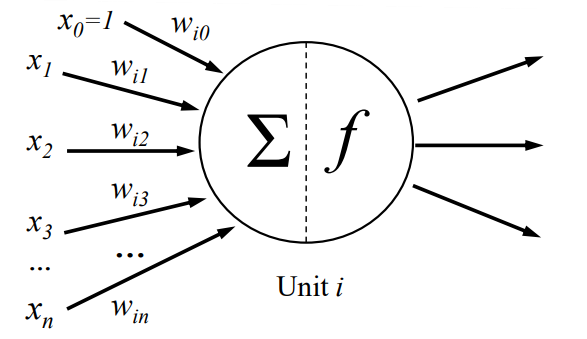
\includegraphics[scale=0.75]{6.png}
\end{center}
Three types of activation functions:
\begin{list}{}{}
	\item \textbf{Linear}, or identity: $f(x) = x$
	\item \textbf{Threshold}, for the \textbf{perceptrons}: $f(x) = sign(x)$
	\item \textbf{Logistic}: $f(x) = \frac{1}{1 + e^{-\alpha x}}$
\end{list}
\paragraph{Perceptron} A neuron that uses a threshold as activation function. Can be composed and connected to build a network: \textbf{MLP}, Multi Layer Perceptron 
\subparagraph{Xor} $x_1 \oplus x_2 = x_1\cdot \overline{x_2} + \overline{x_1}\cdot x_2$. Let $h_1 = x_1\cdot x_2, h_2 x_1 + x_2$ then $x_1 \oplus x_2 = \overline{h_1} \cdot h_2$ with $\wedge = \cdot$ and $\vee = +$.\\
So two layers are sufficient, but single layer cannot model all functions due to limits of single perceptron and the linear separable problems.
\paragraph{Learning for one unit model} \begin{enumerate}
	\item \textbf{Adaline}, adaptive linear neuron: LMS direct solution and gradient descent solution
	\item \textbf{Perceptron}, non linear: only classificiation\\
	Minimize number of misclassified patterns, find $w\:|\:sign(w^Tx) = d$. Online algorithm, a step can be made for each input pattern.
	\begin{enumerate}
		\item Initialize weights
		\item Pick learning rate $\eta$ (between 0 and 1)
		\item Until stopping condition (es weights don't change)\\
		For each training pattern $(x, d)$ compute output activation $out = sign(w^T x)$.\\
		If $out = d$ don't change weights, if $out \neq d$ update weights $w_{new} = w + \eta\cdot d\cdot x$ adding $+\eta x$ if $wx\leq 0$ and $d = +1$ or $-\eta x$ if $wx > 0$ and $d = -1$.\\Different form $w_{new} = w + \frac{1}{2}\cdot\eta\cdot (d-out)\cdot x$
	\end{enumerate}
	\textbf{Delta Rule}: the form $w_{new} = w + \eta\cdot d\cdot x$ is the \textbf{Hebbian learning} form, while the form $w_{new} = w + \frac{1}{2}\cdot\eta\cdot (d-out)\cdot x$ is the \textbf{error correction learning} form. It's a recall from LMS: a error correction/delta/Widrow-Hoff/Adaline/LMS rule that changes the $w$ proportionally to the error (target $d -$ output).\\
	In terms of neurons, the adjustment made to a synaptic weight is proportional to the product of error signal and the input signal that excite the synapse. Easy to compute when errors signal $\delta$ is directly measurable (meaning that we know the desired response for each unit).
\end{enumerate}
\paragraph{Perceptron Convergence theorem} A perceptron can represent linear decision boundaries, so it can solve linearly separable problems. Also, it can always learn the solution with the perceptron learning algorithm.\\
The \textbf{perceptron convergence theorem} is a milestone: a biologically inspired model with well-defined and proved computational capabilities and proved by a theorem. It states that \textbf{the perceptron is guarateed to converge} (classifying correctly all the input patterns) \textbf{in a finite number of steps if the problem is linearly separable}. This independently of the starting point, although the final solution is not unique and it depends on the starting point.
\subparagraph{Preliminaries} We focus on positive patterns, assuming $(x_i, d_i)\in$ TR set with $d_i = +1$ or $-1$. We also omit $^T$ for the dot product $w^T x$ (sometimes).\\
Linearly separable $\Rightarrow\exists\: w^*$ solution $|\:d_i(w^* x_i)\geq \alpha = \hbox{min}_i\:d_i(w^*x_i) > 0$, henche $w^*(d_ix_i)\geq \alpha$.\\
With $x_i' = (d_ix_i)$ then $w^*$ solution $\Leftrightarrow w^*$ solution of $(x_i', +1)$\\
This because $w^*$ solves $\Rightarrow d_i(w^*x_i) \geq \alpha \Rightarrow (w^*d_ix_i)\geq\alpha\Rightarrow (w^*x_i')\geq\alpha \Rightarrow w^*$ solution of $(x_i', +1)$.\\
And if $w^*$ is a solution of $(x_i', +1)\Rightarrow(w^*d_ix_i)\geq \alpha\Rightarrow d_i(w^*x_i)\geq \alpha\Rightarrow w^*$ solves for $x_i$\\\\
Also assuming $w(0) = 0$ (at step $0$), $\eta = 1$ and $\beta = \hbox{max}_i |x_i|^2$ where $|\:|$ is the euclidean norm.\\
After $q$ errors (all false negatives), $w(q) = \sum_{j=1}^q x_{ij}$ with $_{ij}$ denoting the patterns belonging to the subset of misclassified patterns.
\subparagraph{Proof} The basic idea is that we can find lower and upper bound to $|w|$ as a function of $q^2$ steps (lower bound) and $q$ steps (upper bound) $\Rightarrow$ we can find the number of steps $q\:|$ the algorithm converges.\\
Lower bound on $|w(q)|$ is $w^* w(q) = w^*\sum_{j=1}^q x_{ij}\geq q\alpha$ recalling that $\alpha=\hbox{min}_i\:(w^*x_i)$. With Cauchy-Schwartz we know that $(wv)^2 \leq |w|^2|v|^2$ where $|w|^2 = ||w||_2 ^2$.\\
$|w^*|^2|w(q)|^2 \geq (w^*w(q))^2 \geq (q\alpha)^2 \Rightarrow |w(q)|^2 \geq \frac{(q\alpha)^2}{|w^*|^2}$. Also $|w(q)|^2 = |w(q-1)+ x_{iq}|^2 = |w(q-1)|^2 + 2w(q-1)x_{iq} + |x_{iq}|^2$ because $|a + b|^2 = |a|^2 + 2ab + |b|^2$\\
For the $q$-th error, $2w(q-1)x_{iq} < 0$, so $|w(q)|^2 \leq |w(q-1)|^2 + |x_{iq}|^2$ and by iteration $w(0) = 0$ we have $|w(q)|^2 \leq \sum_{j=1}^q |x_{ij}|^2 \leq q\beta$ with $\beta = \hbox{max}_i |x_i|^2$.\\\\
So we have an upper bound $q\beta$ and a lower bound $\frac{(q\alpha)^2}{|w^*|^2}$, so $$q\beta\geq |w(q)|^2\geq \frac{(q\alpha)^2}{|w^*|^2}$$ $$q\beta\geq q^2\alpha'$$ $$\beta\geq q\alpha'$$ $$q \leq \frac{\beta}{\alpha'}$$
\paragraph{Differences}
	$$w_{new} = w + \eta(d-\hbox{out})x$$
Apparently similar but:
\begin{multicols}{2}
	\begin{list}{}{\textbf{LMS algorithm}}
		\item LSM rule derived without threshold activation functions
		\item Hence for training $\delta = d - w^Tx$
		\item Can still be used for classification using\\$h(x) = sign(w^T x)$, LTU
		\item Minimizes $E(w)$ with out = $w^Tx$
		\item Asymptotic convergence also for not linear separable problems
		\item Not always zero classification errors
		\item Can be extended to network of units (NN) using the gradient based approach
	\end{list}
	\begin{list}{}{\textbf{Perceptron learning algorithm}}
		\item Perceptron uses out $= sign(w^Tx)$
		\item versus $\delta = d - sign(w^Tx)$
		\item
		\item Minimizes misclassifications (out = $sign(w^Tx)$)
		\item Always converges in a finite number of steps for a linear separable problem to a perfect classifier\\
		Else it doesn't converge
		\item 
		\item Difficult to be extended to network of units (NN)
	\end{list}
\end{multicols}
\paragraph{Activation functions}
\begin{list}{}{}
	\item \textbf{Linear}, or identity: $f(x) = x$
	\item \textbf{Threshold}, for the \textbf{perceptrons}: $f(x) = sign(x)$
	\item \textbf{Logistic}: $f(x) = \frac{1}{1 + e^{-\alpha x}}$\\
	This is a non-linear squashing function like the sigmoidal logistic function: it assumes a continuous range of values in the bounded interval $[0,1]$. It has the property of being a smoothed differentiable threshold function, with $\alpha$ being the slope parameter of the sigmoid function.
	\item \textbf{Radial basis}: $f(x) = e^{-\alpha x^2}$
	\item \textbf{Softmax}
	\item \textbf{Stochastic neurons}, where the output is +1 with probability $P(net)$ or -1 with $1-P(net) \Rightarrow$ Boltzmann machines and other models rooted in statistical mechanics.
\end{list}
For the derivatives, a step function has no derivative, which is exactly why it isn't used. The sigmoids have\\$\frac{df_\sigma(x)}{dx} = f_\sigma(x) (1-f_\sigma(x))$ and $\frac{df_{tanh}(x)}{dx} = 1 - f_{tanh}(x)^2$ for $\alpha = 1$.\\
The sigmoid logistic function has the property of being a smoothed \textit{differentiable} threshold function. Hence, we can derive a Least (Mean) Square algorithm, by computing the gradient of the mean square loss function as for the linear units (also for a classifier).\\
From $\sigma(x) = x^Tw$ to $\sigma(x) = f_\sigma(x^Tw)$ where $f_\sigma$ is a logistic function. Find $w$ that minimizes the residual sum of squares $$E(w) = \sum_p (d_p - \sigma(x_p))^2 = \sum_p (d_p - f_\sigma(x_p^Tw))^2$$
$$\frac{\partial E(w)}{\partial w_j} = -2\sum_p^l (x_p)_j (d_p - f_\sigma(x_p^Tw))f'_\sigma(x_p^Tw) =$$ $$= -2\sum_p^l(x_p)_j\delta_pf'_\sigma(\hbox{net}(x_p))\hbox{ for 1 unit and patterns }p = 1\ldots l$$
\paragraph{Gradient descent algorithm} 
The same as for linear units using the new delta rule $w_{new} = w + \eta\cdot\delta_p\cdot x_p$ where $\delta_p = (d_p - f_\sigma(net(x_p)))f'_\sigma(net(x_p)) = (d_p-out(x_p))f'_\sigma$
\paragraph{Neural Network} In an MLP architecture: units connected by weighted links, organized in layers:
\begin{list}{}{}
	\item input layer, source of the input $x$. Copies the source external input patterns $x$, without computing $net$ and $f$.
	\item hidden layer, projects onto another hidden or an output layer, computing.
\end{list}
Can be viewed as network of units o flexible function:
$$h(x) = f_k\left(\sum_j w_{kj}f_j\left(\sum_i w_{ji}x_i\right)\right)$$
As for notation, given
\begin{center}
	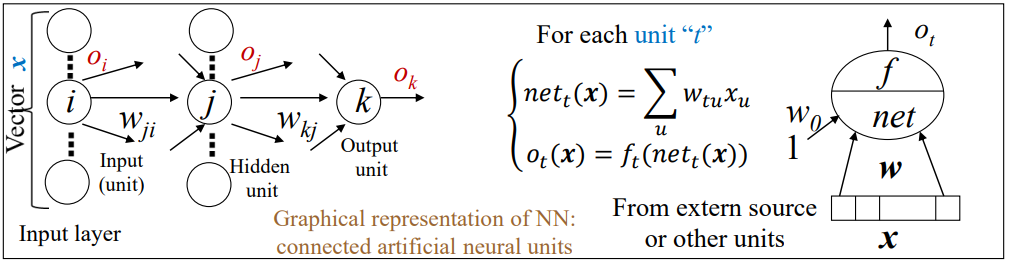
\includegraphics[scale=0.6]{7.png}
\end{center}
We have that the index $t$ denotes a generic unit, can be either $k$ or $j$. $u$ denotes a generic input component, either $i$ or $j$.\\
$x$ is a generic input from an external source (input vector) or from other units according to the position of the unit in the network. If we load the pattern $x$ in the input layer, we can use the notation with $o$ for both the inputs and the hidden units outputs. Hence, inside the network, the input to each unit $t$ from any source $u$ (through the connection $w_{tu}$) is typically denoted as $o_u$.
\subparagraph{Architectures}
\begin{list}{}{}
	\item \textbf{Standard feedforward NN} %TODO ML-21-NN-part1-v.0.1.pdf p.55
\end{list}
\end{document}